\documentclass[twoside,11pt]{article}

% Any additional packages needed should be included after jmlr2e.
% Note that jmlr2e.sty includes epsfig, amssymb, natbib and graphicx,
% and defines many common macros, such as 'proof' and 'example'.
%
% It also sets the bibliographystyle to plainnat; for more information on
% natbib citation styles, see the natbib documentation, a copy of which
% is archived at http://www.jmlr.org/format/natbib.pdf

\usepackage{jmlr2e}
\usepackage{setspace}

% Figures (tables)
\usepackage{float}
\usepackage{caption}
\captionsetup{skip=0pt}{justification=centering}
\usepackage{subcaption}

% Graphics
\usepackage{graphicx}
\graphicspath{{images/}}

% algorithms
\usepackage{algorithmic}

% Proper double quote formatting
\usepackage{csquotes}

% Definitions of handy macros can go here
\newcommand{\dataset}{{\cal D}}
\newcommand{\fracpartial}[2]{\frac{\partial #1}{\partial  #2}}

% Short headings should be running head and authors last names
\ShortHeadings{Dissertation Critique}{Jeschke}
\firstpageno{1}

\begin{document}

\title{Dissertation Critique: Exploring Machine Learning Techniques Using Patient
      Interactions In Online Health Forums to Classify Drug Safety}

\author{\name Christopher Jeschke \email cjeschk2@jhu.edu \\
       \addr Engineering for Professionals\\
       Johns Hopkins University\\
       Elkridge, MD 20175, USA}

\editor{n/a}

\maketitle


% Entire paper should be single spaced
\singlespacing

% Abstract
\begin{abstract}%   <- trailing '%' for backward compatibility of .sty file
  Patient generated health data represents an area of active research interest
  for potential applications in improving the public health. Dr. Brant Chee's 2011 dissertation applying machine learning techniques to patient messages in online health forums explores how watch list drugs from the United States Food and Drug Administration's pharmacovigilance program can be detected via these forum messages.
\end{abstract}

\begin{keywords}
  Drug Safety, Pharmacovigilance, NLP
\end{keywords}

\section{Summary of Research}
Dr. Brant Chee's 2011 dissertation \textit{Exploring Machine Learning Techniques Using
Patient Interactions in Online Health Forums to Classify Drug Safety} describes
Chee's research in applying natural language processing (NLP) techniques in conjunction with Na\"ive Bayes and Support Vector Machine classifiers to identify candidate \textit{watch list} drugs from online patient forums. Watch list drugs are identified by the United States Food and Drug Administration (FDA) as presenting a significant health or safety risk to drug consumers, prompting regulatory action to better inform the consumer or direct intervention by removing the drug from market. Chee's dissertation seeks to answer the specific questions:
\begin{itemize}
  \item Can Machine Learning classification methods using text features extracted from online health forums be used to identify FDA watchlist drugs?
  \item Is the sentiment of the forum message useful in identifying these drugs?
  \item Similarly, are the drug effect entities useful in identifying watchlist drugs?
\end{itemize}

This research is accomplished through an empirical study using a corpus from the
Yahoo! public health forums. Chee develops NLP techniques to define and distill a feature space for classification using Na\"ive Bayes and
Support Vector Machine classifiers for detecting watchlist drugs. Drugs detected are evaluated against watchlist drugs found via the FDA Adverse Event Reporting System (FAERS) to determine the utility of the approach and its applicability in Pharmacovigilance. %GOOD

\subsection{Background: Pharmacovigilance, AERS and Social Media}
The dissertation begins with an extensive background discussion on adverse drug reactions and current surveillance techniques. Adverse drug reactions are defined by the World Health Organization (WHO) as ``a response to a drug which is noxious and unintended and which occurs at doses normally used in man for prophylaxis, diagnosis, or therapy of disease or for modification of physiological function'' \cite{WHO}. Chee continues by introducing Pharmacovigilance as ``the study of drugs once released to market'' \citep{Chee}, and the important regulatory agencies practicing it are mentioned - the WHO and United States Food and Drug Administration (FDA). The FDA Adverse Event Reporting system (AERS) is discussed and comparison with it is central to the work. AERS was constructed to house mandatory drug safety reports from drug manufacturers, distributors and health care facilities, as well as voluntary reports submitted by patients, physicians and other healthcare providers.
Chee identifies a major limitation in AERS and other \textit{spontaneous reporting systems} in that they are known to have high underreporting rates. Social media provides a venue for patients to share their health information in anonymous setting as patients are neither always transparent nor truthful with their physicians. Online health forums create an environment where patients can find those having similar backgrounds, conditions and challenges, prompting rich social interactions where patient disclose their current drug regimen effectiveness and experiences. Chee feels these forums represent an untapped means to crowd source data for the pharmacovigilance task. %Reviewed

\subsection{Experimental Data}
The data selected for the dissertation's experimentation is a Yahoo! corpus containing 12.5 million messages from various Yahoo Health group forums. As the data is a raw export containing a combination of message metadata, raw text and HTML, it must first be studied to better understand its composition and what NLP techniques will be applied for feature extraction. %Reviewed

\subsubsection{Tokenization Study of Data}
Chee conducts an initial study of the Yahoo! corpus by selecting at random 500 messages, stripping them of html tags, numerical and punctuation only tokens (\$, \%, :), :(, et.), then tokenizing them on white spaces with trailing punctuation. The tokens are evaluated in several rounds of classification using lexicons constructed by Chee. Lexicons for English and foreign language were drawn from the OpenOffice project \citep{OpenOffice}, drug names from the Drugs@FDA website, medical and disease terminology from terms on MedicineNet and Wikipedia, and a reactions lexicon from the MedDRA terminology in AERS. A names lexicon was constructed using person names harvested from various sources. The classification process was iterative. If a token did not initially classify via a lexicon, it was manually classified into \textit{error types}. Table \ref{table1} shows average metric counts across the sampled messages:
\begin{table}[H]
  \centering
  \caption{Average Token Counts}
  \label{table1}
  \begin{tabular}{||c|c||}
    \hline
    \verb|Average # of Tokens per Message:| & 172.21\\
    \hline
    \verb|Average # of Drug Name Tokens:| & .29\\
    \hline
    \verb|Average # of Error Type Tokens:| & 7.09\\
    \hline
    \verb|Average # of Name Tokens:| & 5.34\\
    \hline
    \verb|Average # of Medical Tokens:| & .81\\
    \hline
  \end{tabular}
\end{table}
Of the error tokens, over 54\% of them were found to be foreign language tokens, motivating experimentation to classify messages as English before incorporating them into later studies. Spelling errors were also a concern, but the classification results show only a $.8\%$ error rate. %Reviewed.

\subsubsection{A Vocabulary for Experimentation}
Chee cites performance concerns training classifiers using all the words in the message, as this would expand the feature space. Multiple words together in order can convey a different meaning than separate single words motivating the use of word-grams - unigrams, bigrams and trigrams - to capture meaning. Therefore, specialized lexicons are developed to ensure the classifiers do not over fit to drug names and generalize to considering drug effects, sentiment and other terminology. The lexicons are:
\begin{itemize}
  \item drugs - a drug list from drugs.com
  \item medical - medical terminology extracted from MedicineNet
  \item sentiment - a sentiment lexicon from the combination of SentiWordNet and Linguistic Inquiry and Word Count (LIWC)
  \item medra - the MedDRA terms for drug adverse events/outcomes from FDA AERS
  \item disease - a disease list from Wikipedia
\end{itemize}

\subsection{Language Identification for Messages}
The tokenization study identified a significant number of foreign language messages, which Chee seeks to eliminate to reduce the feature space. Messages containing non-Romanized text are removed first using Unicode language detection. Messages in non-English languages in Romanized text are harder to discern. Dictionaries for English and foreign languages are taken from the OpenOffice project and used in conjunction with the medical and drug lexicons mentioned earlier obtain token counts. Once the counts are obtained, the following linear inequality is evaluated per message:
\[
  4 * foreign + unknown + ignore > english + drugs + medical
\]
The weighting of the foreign words is selected to ensure messages contain less than 25\% foreign words to be considered English. Only the English messages are retained, reducing the corpus to 10,178,710 messages and the number of unique terms per message from 2.5 to 2. %Reviewed

\subsection{Experimentation and Results}
The goal of the dissertation is to develop a classification system for drugs based on how people are talking about them in online message forums. Chee constructs a multitude of experiments using various classifier & lexicon combinations and other options to deduce the best classifier configuration(s) for use in the final system.

\subsubsection{Class Separability}
Chee begins with an experiment to determine how separable messages about watchlist and non-watchlist drugs are. Kullback-Leibler divergence (KL Divergence) is used to measure the difference in word frequency distribution between messages in each class. Table \ref{table2} shows the divergence between classes, as well as divergence from Google and Reuters corpi to provide perspective. Terms overexpressed in watchlist messages are in Table \ref{table3}:
% Two tables side by side
\begin{minipage}{0.75\textwidth}
  \begin{table}[H]
    \caption{Class Divergence}
    \label{table2}
    \begin{tabular}{||c|c|c|c|c||}
      \hline
      Class & Watchlist & Non-Watchlist & Google & Reuters \\
      \hline\hline
      Watchlist & n/a & .1684 & 1.4178 & 1.3279 \\
      \hline
      Non-Watchlist & .1778 & n/a & 1.1804 & 1.0815 \\
      \hline
    \end{tabular}
  \end{table}
\end{minipage}
\begin{minipage}{0.25\textwidth}
  \begin{table}[H]
    \caption{Terms}
    \label{table3}
    \begin{tabular}{||c|c||}
      \hline
      Term & Divergence \\
      \hline\hline
      i & .007875 \\
      \hline
      my & .003018 \\
      \hline
      me & .0002256 \\
      \hline
      you & .001712 \\
      \hline
      i'm & .000964 \\
      \hline
    \end{tabular}
  \end{table}
\end{minipage}

Clearly watchlist and nonwatchlist diverge, and show a different degree of divergence from the Google and Reuters corpi. The overexpressed terms are interesting, as they seem indicative of emotional writing - just the kind that might occur when discussing a drug with an adverse effect.

\subsubsection{Named Entity Recognition in Messages}
Another challenge presented is how to identify the drugs and adverse events in a message - a problem of Named Entity Recognition (NER). A Lucene index is built atop the messages, against which query phrases built from the drug and reactions lexicons are issued to determine term prevalence. A lower case filter with stemming is used, requiring that drugs containing common words (e.g. ``commit'' for the drug Commit) be replaced with their generic chemical names in the lexicon. Plots are produced showing term distributions:

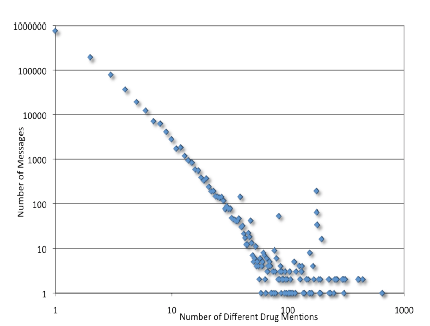
\includegraphics[width=7cm, height=5cm]{Figure-1-Zipfian.png}
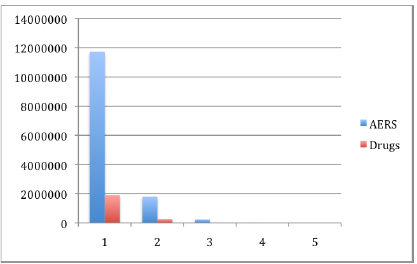
\includegraphics[width=7cm, height=5cm]{Figure-2-AERS_Drugs.png}

The first plot demonstrates a Zipfian distribution for drug name mentions in the messages, with more than 96\% of messages mentioning at most 5 drugs, prompting the elimination of messages with more than 5 unique drugs. The second plot shows adverse events are mentioned far more often than drug names, a cause for data scarcity concern. If multiple drugs are mentioned in a single message it becomes difficult to discern which drug the message should apply to, so another study is done to evaluate the number of characters between the top 25 co-occurring drugs. A Zipfian distribution is observed again, suggesting drugs are talked about within the same or adjacent sentences, making separation difficult. Chee defaults to attributing each message to all drugs mentioned.

\subsubsection{Sentiment Feature}
 Chee hypothesizes the degree of negative valence in a message represents drug satisfaction, making it an interesting feature to incorporate into classification. A lexicon using terms from Linguistic Inquiry and Word Count (LIWC) is constructed, augmented with emoticons and acronyms. Two case studies are executed using messages sampled from specific groups in the corpus. The change in drug sentiment is analyzed over the drug's pre-recall, recall, and post-recall timeframes against a control sentiment derived from messages not containing the drug.

\begin{minipage}{.5\textwidth}
  \begin{figure}[H]
    \caption{Tysabri}
    \label{fig:tysabri}
    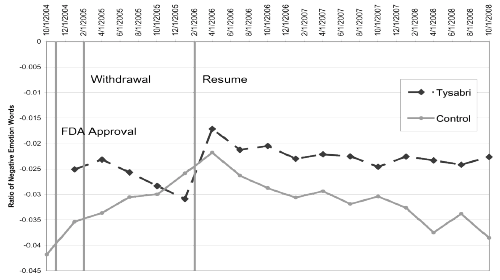
\includegraphics[width=7.5cm, height=6cm]{Figure-3-Tysabri.png}
  \end{figure}
\end{minipage}%
\begin{minipage}{.5\textwidth}
  \begin{figure}[H]
    \caption{Vioxx}
    \label{fig:vioxx}
    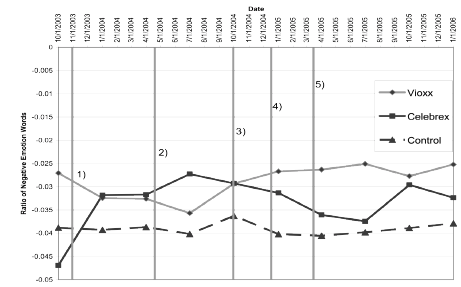
\includegraphics[width=7.5cm, height=6cm]{Figure-4-Vioxx.png}
  \end{figure}
\end{minipage}

Figure \ref{fig:tysabri} shows a reasonably intuitive change in negative valence for Tysabri when it is introduced (more positive), withdrawn (negative), reintroduced (hopeful therefore positive), finally stabilizing. Figure \ref{fig:vioxx} shows sentiment change for a pair of commonly used pain relievers - Vioxx and Celebrex - over the course of several public anouncements. First a withdrawal of Viox (sections 1 through 3), then Celebrex (4 and 5). ANOVA is applied, determining statistical significance against the control with \verb|p < .001|.

\subsubsection{Feature Selection, Training and Test Data Size}
The introduction to the main body of classification experiments is preceded by a brief discussion on the features vectors used, as well as how cross-validation training is setup. Two types of feature vector are decided upon. The first is generated over general vocabulary terms in the messages selected based on frequency, then augmented with counts from the specialized lexicons. The second feature vector uses only the specialized lexicons to identify the word features.
Training data is of foremost concern, as there are only 435 drugs having 500 or more unique messages, and only 575 drugs having more than 250 messages, with 63 and 77 watchlist drugs mentioned in each respectively. Approximately 90\% of message instances reference non-watchlist drugs, creating a data scarcity problem. Chee decides upon a minimum cutoff of 250 messages per drug. An experiment is constructed to evaluate techniques to address the scarcity: scaling features, selecting different ratios of negative to positive training examples, and experimenting with different split ratios in cross-validation - 90/10 and 80/20. These experiments are deemed inconclusive and not elaborated on further.

\subsubsection{Classifier and Lexicon Selection}
The next goal of the dissertation is to discover the best performing combinations of classifier, lexicons and feature selection as a means to inform the construction of a \textit{Meta classifier} used in watchlist drug prediction. A training methodology is devised where test and training sets are sampled with the same distribution as the original data, divided into a 90/10 split with 90\% of the samples for training and 10\% for validation. The splits themselves mirror follow the original distribution.
The experimental results and analysis make heavy use of acronyms to understand the combinations evaluated. For example, \textit{drugs\_dis\_sent\_react\_NSVMC} would equate to using a Normalized SVM with Cost Weighting (NSVMC) incorporating the drugs(drugs), disease(dis), sentiment(sent) and reaction(react) lexicons. A series of 240 experiments were run using various combinations to ascertain the best configurations for accuracy, F1 score, and area under the ROC curve (AUC). Table \ref{table4} shows the top 3 classifier configurations by accuracy with upper and lower bounds for the 95\% confidence interval:
\begin{table}[H]
  \centering
  \caption{Accuracy}
  \label{table4}
  \begin{tabular}{||c|c|c|c||}
    \hline
    Configuration & Accuracy & Lower & Upper \\
    \hline\hline
    \verb|dis_react_NSVM| & 0.9032 & 0.7932 & 0.9578 \\
    \hline
    \verb|drugs_dis_sent_react_NSVM| & 0.9013 & 0.7908 & 0.9566 \\
    \hline
    \verb|drugs_sent_react_NSVM| & 0.9013 & 0.7908 & 0.9566 \\
    \hline
  \end{tabular}
\end{table}
The accuracy of a na\"ive baseline classifier that labels all instances as negative would be 86.7\% per concentrations of non-watchlist and watchlist drugs in the training data. While several configurations exceed this, the lower bound introduces uncertainty that any classifier is more accurate than the baseline. The F1 and AUC scores are in tables \ref{table5} and \ref{table6} respectively.

\begin{minipage}{.6\textwidth}
  \centering
  \begin{table}[H]
    \caption{F1 Scores}
    \label{table5}
    \begin{tabular}{||c|c||}
      \hline
      Configuration & F1 \\
      \hline\hline
      \verb|drugs_dis_react_NSVM| & 0.4761 \\
      \hline
      \verb|drugs_dis_react_UNB| & 0.4725 \\
      \hline
      \verb|drugs_UNB| & 0.4698 \\
      \hline
    \end{tabular}
  \end{table}
\end{minipage}
\begin{minipage}{.4\textwidth}
  \centering
  \begin{table}[H]
    \caption{AUC}
    \label{table6}
    \begin{tabular}{||c|c||}
      \hline
      Configuration & AUC \\
      \hline\hline
      \verb|drugs_UNB| & 0.7592 \\
      \hline
      \verb|drugs_dis_UNB| & 0.7564 \\
      \hline
      \verb|med_drugs_NNB| & 0.7545 \\
      \hline
    \end{tabular}
  \end{table}
\end{minipage}


Neither the F1 nor AUC scores are particularly impressive. The F1 scores were decomposed into their precision and recall components, and scatter plotted. A general observation was most scores had a mass concentration of low recall and precision, with the occasional high recall or high precision outlier - though never both.

\subsubsection{Evaluating the BNS Lexicon}
Bi-Normal Separation (BNS) is an alternative technique explored by Chee for discovering the word n-grams. BNS identifies those n-grams that are differentially expressed between two classes. BNS lexicons are constructed using the test subset of data for the top 15,000, 10,000 and 5,000 word n-grams, then tested in combination with the drugs, disease and sentiment lexicons, as well as additional ``numerical features'' containing counts of terms hits into each lexicon. Unfortunately the best BNS classifier underperformed the previous tests with an accuracy of only .8762 and lower bound of .7602. The F1 and AUC scores for this test showed no improvement either, dismissing the value of BNS and the additional features.

\subsubsection{Predicting Watchlist Drugs}
The previous experiments were used to assemble a meta-classifier using the best classifiers based on accuracy, F1 and AUC scores. A normalized SVM with the disease and reaction lexicons is selected for its 90.33\% accuracy. The normalized SVM with drug, disease and reaction lexicons is selected for its F1 score of 0.4762. Finally, an Un-normalized Na\"ive Bayes with the drugs lexicon is used for its AUC score of 0.7925.
Two meta-classification experiments are constructed. The first experiment uses training data modified to denote drugs \textit{withdrawn} from the market as non-watchlist, as withdrawn drugs represent a subclass of watchlist drugs. By looking for these non-watchlist, withdrawn drugs in the false positives from the results, we evaluate the ability to discern new watchlist drugs. This experiment was executed via training runs to build 100 classifiers of each configuration. A scoring methodology is applied using the following linear combination $\frac{fp}{occurrences} * fp * (classifiers)$, where $fp$ is a \textit{false positive}, an occurrence is an instance of a withdrawn drug being classified, and classifiers is a count of the unique classifiers generating a positive classification. Table \ref{table7} below shows the top 5 scores by generic drug name, as well as those withdrawn drugs identified as false positives.
\begin{table}[H]
  \centering
  \caption{Withdrawn drugs marked non-watchlist}
  \label{table7}
  \begin{tabular}{||c|c|c|c|c||}
    \hline
    Drug & # Positives & # Occurrences & # Classifiers & Score \\
    \hline\hline
    \textit{clozapine} & 31 & 64 & 3 & 45.047 \\
    \hline
    \textit{fludarabine} & 29 & 61 & 3 & 41.361 \\
    \hline
    \textit{methylphenidtate}(Ritalin) & 25 & 50 & 3 & 37.500 \\
    \hline
    \textit{morphine} & 15 & 38 & 3 & 15.474 \\
    \hline
    \textit{meloxicam} & 15 & 50 & 3 & 13.500 \\
    \hline\hline
    \textit{thalidomide} & 10 & 36 & 1 & 2.778 \\
    \textit{temazepam} & 11 & 50 & 1 & 2.420 \\
    \textit{hydromorphone} & 9 & 42 & 1 & 1.929 \\
    \textit{trovafloxacin} & 9 & 46 & 1 & 1.761 \\
    \textit{rofecoxib} & 9 & 50 & 1 & 1.620 \\
    \textit{sibutramine} (Meridia) & 5 & 27 & 1 & 0.926 \\
    \textit{cerivastatin} (Baycol) & 1 & 33 & 1 & 0.030 \\
    \hline
  \end{tabular}
\end{table}
The generic Sibutramine (brand name: Meridia) is of particular interest to this study, as it is under review but not yet an official watchlist drug. FDA has issued safety communications as of November of 2009, and the European Union has removed it from the market.
The second experiment entails removing the withdrawn drugs entirely from training, classifying them after a classifier is built for each fold during cross-validation. This approach is presumed to identify the withdrawn drugs with greater confidence as they are not present in the training data. Table \ref{table7} shows the results.
\begin{table}[H]
  \centering
  \caption{Withdrawn drugs removed}
  \label{table7}
  \begin{tabular}{||c|c|c|c|c||}
    \hline
    Drug & # Positives & # Occurrences & # Classifiers & Score \\
    \hline\hline
    \textit{methlyphenidate} (Ritalin) & 30 & 34 & 3 & 79.412 \\
    \hline
    \textit{morphine} & 13 & 38 & 3 & 13.342 \\
    \hline
    \textit{questiapine} & 14 & 31 & 2 & 12.645 \\
    \hline
    \textit{indomethacin} & 19 & 37 & 1 & 9.757 \\
    \hline
    \textit{sibutramine} (Meridia) & 17 & 34 & 1 & 8.500\\
    \hline\hline
    \textit{trovafloxacin} & 33 & 100 & 1 & 10.89\\
    \hline
    \textit{hydromorphone} & 33 & 100 & 1 & 10.89\\
    \hline
    \textit{rofecoxib} & 32 & 100 & 1 & 10.24 \\
    \hline
    \textit{thalidomide} & 10 & 36 & 1 & 2.778\\
    \hline
    \textit{temazepam} & 8 & 28 & 1 & 2.286\\
    \hline
    \textit{cerivastatin} (Baycol) & 2 & 100 & 1 & 0.04\\
    \hline
  \end{tabular}
\end{table}
Interestingly sibutramine does score significantly higher in this experiment, as do several of the withdrawn drugs (hydromorphone, rofecoxib, trovafloxacin). Psychiatric drugs (Ritalin) and opiates (morphine) show up near the top in both experiments, presumably because they are more dangerous and more often associated with adverse reactions.

\section{Discussion of Contributions}
The major contribution of the dissertation is a collection of techniques for leveraging public health forum data for pharmacovigilance. Techniques in natural language processing and classification are developed and applied to identify drugs withdrawn from the market by the FDA by using only the textual features of the messages themselves. The end result was an ensemble classification technique capable of identifying future watchlist drugs. In the interest of discussion, we can distill this work into several specific contributions worth individual discussion.

\subsection{Exploration and Annotation of Health Forum Data}
Chee's initial exploration exposes the challenges in annotating messages from the general public for use in a scientific study. Message content must be differentiated from HTML tags, garbage strings and web URLs nested within. Colloquial language, abbreviations and slang challenge determining sentiment and discovering medical terminology. Misspellings may disproportionately impact medical terms because of their complexity.
\par The majority of message tokens contributing to these problems were placed in a general category of \textit{error}, prompting a more in depth exploration into the nature of the errors and discovering that foreign languages are the largest contributor. However, the methods here did not go much further than identifying that problem tokens were present. If a problem token was capable of being classified manually, why not replace it with a grammatically correct token of equivalent meaning? Modern word processors frequently correct for misspellings and slang terminology such as ``sux'' could be replaced by a working equivalent. Furthermore, these token statistics used only 500 messages, which is .004\% of the original corpus. The automated analysis might have been more valuable if extended to the whole corpus.

\subsection{Techniques for Differentiating Language}
Foreign language is concerning, as these terms can inflate the word n-gram feature vector size going into the classifiers. Chee starts by using Unicode language detection to take advantage of the most common website text representation: UTF-8, thereby eliminating some non-English messages. Next, simple dictionary based methods using lexicons drawn from OpenOffice are used to classify tokens in a message as English for use in message scoring. Chee mentions the common words technique and n-gram based techniques, but dismisses the later as requiring non-existent training data.
\par Dunning \citep{Dunning} gives attention to the common words technique, stating these techniques are suitable when enough text is present to be classified as the common words are often \textit{closed class} words, with examples such as: and, or, this, that. These words serve a function, such as joining other words and phrases, providing structure to text. Sufficient amounts of text allow this structure to be identified and leveraged in classification. Dunning uses counter examples that are 20-characters long and 3-4 tokens to highlight the limitation, but considering the average 172 token length of the Yahoo! corpus it might have been more informative had Chee explored this technique further.
\par Dunning's n-gram language classification technique would have been worth applying to develop a binary english-non-english classifier. Dunning develops his classification technique by modeling languages as a Markov Decision Process, where the probability of a particular word or phrase is dependent upon those preceding it and their probabilities assume a specific language. Dunning successfully differentiates between English and Spanish texts of small length: 10, 20, 50, 100 and 200 bytes, having used relatively small training texts between 1000 and 50000 bytes. This would be a small training corpus to compose.
\par Recall the inequality $(4 * foreign) + unknown + ignore > english + drugs + medical$ used in message classification. Only the ~18.7\% reduction in message count thanks to the technique is provided as evidence of effectiveness. The algorithm used by Chee begins by checking for token presence in the English lexicons \textit{first}, incrementing the foreign token count only the token isn't found. The vocabulary of the English language has been highly influenced by French and Germanic languages \citep{English}, accounting for more than 55\% of the words. This approach seems vulnerable to misclassification. While language classification is cited as a contribution of the dissertation, the utility of this approach is questionable.

\subsection{Named Entity Recognition: Drugs and Drug Effects}
Chee again favors dictionary methods for identifying drugs and drug effects within messages. The reactions lexicon is composed the Medical Dictionary for Regulatory Activities (MedDRA) terms used when coding reactions in the reports \citep{FAERS}. MedDRA has an ontological structure characterized by a top-most level of ``System Organ Classes'' (SOCs), two intermediate levels of high-level terms falling within a SOC, followed in the lowest levels by a preferred term (PT) and its synonyms, lowest level terms (LLT). It is the LLT or PT that may be recorded in an AERS report. Preferred terms are typically clinically correct (Nausea), with the LLT being a more relaxed, colloquial phrase (feeling queasy). The number of AERS (MedDRA) term instances found across the Lucene indexed corpus of ~10M messages was 13,794,445 and the NER study indicated at least 1 reaction per message, indicating this may be a useful technique for identifying adverse reactions in messages.
\par The results for drug identification were less promising.  The drug lexicon was composed from the FDA and a drugs taxonomy on Drugs.com. Chee outright states limitations in this approach as it does not account for all therapeutic biologicals, foreign names of drugs, nor the names of drugs not approved for US use. Drugs with brand names containing common words (ex: Commit) present a problem, as do colloquial or slang terms. The volume of drug mentions was considerably less than the total number of messages, at 2,228,588. Without a broader lexicon, it is difficult to claim this method is successful at identifying drugs in messages. Low volume of drug identification in messages is one of the chief limitations of the work, in that very few watchlist drugs (77) were found, restricting the volume of training data.

\subsection{Feature Generation using BNS, Specialty Lexicons}
Bi-Normal Separation (BNS) experimentation was intended to determine if word features (n-grams) expressed differently between watchlist and non-watchlist messages could serve as useful classification features. A study by Forman \citep{Forman} showed strong preference to BNS for feature identification in text classification for its ability to deduce word features occurring with greater prevalence in one class versus another. Counter intuitively the BNS experiments actually showed worse results compared to the use of the specialized lexicons by themselves.
\par Methodological concerns were identified that may have contributed to this. First, Chee notes that the BNS term lexicons were constructed using the test subset of the data, representing only 10\% of the messages. This was done to avoid biasing the classifier to the Yahoo! corpus, but at the same time significantly reduced the sample size. Secondarily, the BSN terms were used in addition to the specialty lexicons. At no point do we get to evaluate BNS selected n-grams in isolation.
\par The sentiment lexicon was another disappointment. While isolated evaluation with certain drugs (Tysabri, Vioxx) showed changes in negative valence with watchlist status, its importance in the top classifiers was still outshone by drug and disease lexicons. This is concerning because those lexicons could cause a classifier to over fit to drug names, hindering its ability to predict new watchlist drugs. Overall, the dissertation seems to have been unsuccessful in finding a clear set of word features to separate watchlist from non-watchlist drugs.

\subsection{Quality of Watchlist Predictions}
Initially one would not be satisfied with the minimal difference in accuracy shown between a naive classifier classifying each drug as non-watchlist (86\%) versus the accuracy observed in some of the best trained SVMs (90\%). F1 and AUC scores were not exciting either. However, consider how these scores are defined:
\[
  Accuracy = \frac{TP + TN}{TP + TN + FP + FN}
\]
\[
  F1 = 2 \cdot \frac{precision * recall}{precision + recall}, \ precision = \frac{TP}{TP+FP},\ recall = \frac{TP}{TP+FN}
\]
\[
  AUC = P(X_{1} > X_{0})
\]
TP, TN, FP, FN stand for true positive, true negative, false positive and false negative respectively. For AUC, $X_{0}$ and $X_{1}$ are the classifier scores of randomly chosen positive and negative instances, therefore an AUC = 1 represents perfect classification. A naive classifier assuming all instances were negative (non-watchlist) would have AUC and F1 scores of 0 and contribute nothing towards the goal of discovering future watchlist drugs. Note that each performance metric places value on the distinction between a true positive and a false positive, yet false positives are the means by which the value of the approach is communicated. Drugs do not become watchlist drugs until labeled so by the FDA. It might have been interesting had Chee experimented with those classifiers having the highest \textit{recall} rates and evaluated the quality of the false positives raised.
Chee's technique was successful in identifying a number of drugs withdrawn from the market despite their having been labeled as non-watchlist:  Palladone,  Trovan, Vioxx, and Baycol. The discovery of \textit{Sibutramine} (Meridia) was compelling because the time frame of the data set used stopped one year before Meridia was placed on a watchlist, demonstrating the ability to detect future watchlist drugs. It is far better to accidentally label a drug as a false positive, watchlist candidate than mistakenly mark it as false negative, failing to call attention to it and allowing considerable, sometimes-deadly health consequences to go unnoticed.

\section{Techniques and Algorithms}
Summarized herein are the technical details regarding the techniques and algorithms Chee used in his study, particularly as they pertain to feature selection and classification.

\subsection{KL Divergence}
Kullback-Leibler (KL) divergence quantifies the difference between two probability distributions. Given two distributions P and Q, it is expressed as:
\[
  D_{KL}(P||Q) = \sum_{i}P(i)log\frac{P(i)}{Q(i)}
\]
Where $P$ and $Q$ are probability distributions for two classes, $i$ is a value within each class, and $P(i)$ and $Q(i)$ are the probability of $i$ in each distribution respectively. Care must be taken that if $i$ is not present in $Q$, infinite divergence would occur, and so a low, default probability for $Q(i)$ is used by Chee.

\subsection{Bi-Normal Separation}
Bi-Normal Separation (BNS) is introduced as a word feature selection technique for use text classification. An empirical study by \citep{Forman} showed considerable performance advantages when using BNS with SVMs for text classification, as opposed to other selection metrics such as Information Gain (IG), Document Frequency (DFreq) and Odds Ratio (Odds). Testing with BNS had higher F1, precision and recall despite dealing with significant class skew in the training data on the order of 1:31 - 1 positive to 31 negative class examples. The BNS for at term is computed as:
\[
  F^{-1}(tpr) - F^{-1}(fpr)
\]
where $F^{-1}$ is the inverse of the normal cumulative distribution function, $tpr$ and $fpr$ are true and false positive rates for that term in text classes. Special exception is given to $F^{-1}(0)$ by defaulting to 0.0005 to avoid undefined values when a term is not present in one class.

\subsection{Support Vector Machines}
Support Vector Machines (SVM) \citep{Vapnik} are well established for their utility in classification problems. An SVM functions by discovering a hyper plane that maximizes the margin of separation between two classes given their feature space. The simplest SVM finds the optimal hyper plane (w,b) satisfying the inequality:
\[
  y_{i}(w \cdot x_{i} + b) \gte 1,  i = 1, ...., l
\]
Where l = n, the number of training samples, and each training sample is a tuple $(x_{i}, y_{i})$, with $x_{i}$ the feature vector, $y_{i} = 1$ indicates membership of the positive class and $y_{i} = -1$ indicates membership of the negative class. If $(w, b)$ are successfully found we have a \textit{hard margin} SVM classifier. Rarely are classes so perfectly separable, so Chee opts to use a \textit{soft margin} SVM with a \textit{Gaussian Radial Basis Function} (RBF) kernel:
\[
  y_{i}(w \cdot \Phi{x_{i}} + b) \geq 1 - \xi_{i}
\]
The classification error $C\sum_{i=1}^{l} \xi_{i}$ is minimized, with $C$ a penalty parameter. The kernel function $\Phi$ projects $x_{i}$ into a new dimensional space according to the RBF definition $\exp(-\gamma||x_{i} - x_{j}||^{2}),\ \gamma > 0$. The parameters $C$ and $\gamma$ must be specified when training the SVM, so this dissertation utilizes a \textit{grid search} to find the combination yielding the best performance.

\subsection{Naive Bayes Classification}
The fundamental assumption in Na\"ive Bayes is that the features (word n-grams) are independently distributed from one another within the classes of interest. This classification technique seeks to answer the question ``What is the probability that a given document D belongs to class C?}'', expressed as the \textit{conditional probability} $p(C|D)$ - the probability of the class $C$ given the document $D$. Bayes Theorem allows the manipulation of conditional probability to express $p(C|D)$ as:
\[
  p(C|D) = \frac{p(C)p(D|C)}{p(D)}
\]
where $p(D|C) = \prod_{i}p(w_{i}|C)$ with $w_{i}$ representing the $ith$ word in a given document. Consider that we have two classes $C_{wl}$ and $C_{nwl}$ for watchlist and non-watchlist respectively. Watchlist probability would have the following form:
\[
  p(C_{wl} | D) = \frac{p(C_{wl})}{p(D)}\prod_{i}p(w_{i}|C_{wl})
\]
with a comparable rule for non-watchlist. Binary classification in Naive Bayes makes use of a \textit{decision rule}. The \textit{maximum a posteriori} (MAP) rule was selected, which chooses the most probable hypothesis. We are then given a classifier defined as:
\[
  \hat{y} = argmax_{k \element {wl, nwl}} p(C_{k}) \prod_{i=1}^{n}p(x_{i}|C_{k})
\]
$\hat{y}$ is assigned the class label based on the $k$ chosen per the maximization defined above.

\section{Literature Review}

\subsubsection{Health & Safety Literature}
Adverse reactions have long held the attention of health regulatory bodies such as the WHO and FDA. In 1967, the WHO initiated a research project to collect case reports from 10 countries to evaluate an international system for monitoring adverse drug effects \citep{WHO}, prompting the WHO Drug Monitoring Centre - now the Uppsala Monitoring Centre - to establish the first international pharmacovigilance program.

\subsubsection{Text processing}
Rude, Gortner and Pennebaker conducted a study of easy writing by currently depressed, formerly depressed and never depressed college students, with the hypothesis that terms indicating self-preoccupation such as ``I'' will be more prevalent in depressed individuals, as well as emotional terms with negative valence \citep{Rude}. Their study did confirm the hypothesis that ``I'' is used more frequently by currently depressed students, though other pronouns referencing the self were not. The study leveraged the Linguistic Inquiry and Word Count (LWIC) textual analysis program used by Chee in constructing a sentiment lexicon.

Pang and Lee \citep{Pang} discuss the implications of treating online opinions as a first class object - something we actively mine for and take value in. They conduct an extensive survey of approaches for opinion-oriented search geared towards freeform text in blogs and forums, where opinion and sentiment must be deduced directly from message content, without the assistance of meta-data such as rankings (e.g.  1 to 5). Pang and Lee are able to characterize sentiment as a regression problem, as we can characterize a degree of positive and negative sentiment. Extraction of textual features is discussed, comparing the value of term \textit{frequency} versus \textit{presence}, the former usually being term-frequency inverse document frequency (tf-idf) and the later a binary indicator that a word is present or not. Previous studies by Pang indicate the later shows better performance in sentiment classification, differentiating sentiment modeling from topic modeling, likely influencing Chee's approach to sentiment feature modeling.

Named entity recognition (NER) is an area of particular relevance to this work. Extracting drug names, diseases and medical terminology from biomedical text
is addressed by \citep{Rindflesch} through the development of EDGAR, a natural language processing system for discovering drug & gene relationships pertaining to cancer as documented in biomedical literature. EDGAR benefits heavily from using the Unified Medical Language System (UMLS) and MetaMap \citep{Metamap} - an already existing tool for identifying medical language in text. EDGAR leverages contextual elements and consistency in phrase structure to identify gene, cell and drug names, and then constructs relationship predicates between them (e.g. is\_resistant(gene, cell, drug)). However, this approach heavily leverages the grammatical consistency of these texts, making it less applicable for recognizing named medical entities in web data.

General entity recognition in web data is examined in \citep{Etzioni}, where the KnowItAll system is developed and discussed - an unsupervised, domain-independent system for information extraction from the Web. The system uses generalized extraction patterns to generate candidate facts - such as city names - that are then tested for truth using assistance from search engines queries to compute a point wise mutual information statistic for the fact. Chee emulates some of these techniques through phrase queries to validate drug names found in the Yahoo! corpus.

\subsubsection{Technical Literature}
Forman's paper on feature selection metrics for text classification \citep{Forman} introduces the BNS technique, comparing it to several other metrics:  Chi-Squared, Information Gain, Odds Ratio,  Log Probability Ratio, and Document Frequency. Forman's experimental method uses a data set of computer science paper abstracts categorized into classes intermingled with another text classification data set, producing a variety of test data sets having a skew ranging from 1:1 to 1:100+ (more than 100 negative instances). Classification experiments using SVMs are run with the features selected. BNS shows a consistently superior F1 measure and accuracy in the tests, with exception given to IG when the number of features selected is restricted to between 20 and 50 and the class skew is low. Incidentally, Forman's analysis uses SVM only, citing the work of \citep{Joachims} as confirming that SVM is an ``outstanding'' method for text classification.
\par SVMs are introduced by \citep{Vapnik}, introducing fundamental concepts, and hard and soft margin classifiers. Joachim's paper on text categorization with SVMs \citep{Joachim} explains why SVMs are expected to work well for text categorization, highlighting their ability to handle a large feature space of several thousand relevant words where training sample vectors may be sparse. Joachim compares SVM text classification using polynomial and RBF kernels against Na\"ive Bayes, k-NN, C4.5 and the Rocchio algorithm, showing consistently higher precision/recall break even points for the SVMs across two popular test corpus.
\par Na\"ive Bayes classification is explored in the context of SPAM classification by \citep{Sahami}, who evaluates Naive Bayes classifiers trained on combinations of message word features, message word features plus specific phrases, and word features with phrases and domain specific features (non-word) features thought to indicate spam. Classification results in the binary SPAM/no-SPAM setting showing 100\% precision when using the final combination tested on a corpus of 1789 labeled messages. Like other studies, Sahami employs feature selection techniques to manage the feature space, ignoring words that appear less than three times and selecting only the top 500 remaining words based on their mutual information scores relevant to the class labels.

\section{Application Areas}
Chee's techniques seem reasonably applicable as an augmentation to current Pharmacovigilance programs that use structured reporting systems. The opportunity to leverage public health forum data in safety signal detection could help in the earlier identification of watch-list candidate drugs for these programs to pay special attention to when monitoring existing safety systems. A system of monitoring public forums in this fashion could leverage what are a far greater volume of data, and the tendency for people to disclose medical issues and sentiments more readily within peer groups. Public health forum data is not necessarily the only data set where this technique could be applied either. The techniques developed within this dissertation could be applicable to clinical notes in electronic health records, health surveys or similar unstructured data sources, and are potentially extensible to any medical product where adverse reactions could be associated: devices, biologicals (a separate classification of drug), procedures, or named treatment regimens.

Chee's exploration of the Yahoo! corpus message content is illuminating, identifying the difficulties with language recognition, colloquial phrases, and other message artifacts germane to online messaging. The lexicon techniques developed were simple and functional, but would need further development to generalize well. For example, recognizing slang is a compelling problem in its own right and therefore developing slang lexicons for various languages or domains could provide a valuable toolset for normalizing online messages to more grammatically correct text, against which already existing trained, supervised NLP machine learning techniques could be applied, thereby improving named entity recognition capabilities and perhaps the robustness of the overall technique.

Feature selection within the study is another application area to address. It was surprising sentiment did not have a stronger influence in the classification experiments, but the use of the disease and drug lexicons might have over fit trained classifiers to drug names and suppressed any significant contribution from sentiment. Revisiting sentiment as an initial feature to which additional features might be added/removed would be an interesting extension of the study. The case studies mapping sentiment change in known watchlist drugs were insightful and might point to another way of signaling a future watchlist drug. The use of BNS bears revisiting per methodological concerns.

Finally, it is worth discussing that this technique is not limited only to problems in the health and medical domains. Consumer product safety in general could benefit from monitoring public forums in this fashion in order to identify products posing significant safety hazards. Thousands of consumer products for child safety - such as car seats and life jackets - are available for purchase by the general public. Regulatory agencies such as the National Highway Traffic Safety Administration must evaluate products and post recall notifications, but despite best efforts unsafe products will still make it to market. Constructing similar monitoring systems for these agencies using public forums could help identify products in the market with previously unrecognized defects.

\bibliography{dissertation_critique}
\vskip 0.2in
\end{document}
